% ---------------------------------------------------------------------
% §9: Zero-Prefill Keep-Alive Protocol
% ---------------------------------------------------------------------
\setcounter{section}{8}
\section{Zero-Prefill Keep-Alive Protocol}
\label{sec:zero-prefill-protocol}

The Asymmetric Prefill Gateway (APG, \S\ref{sec:polyglot-stack})
maintains the Stochastic Eviction Horizon $\mathcal{H}_{\text{evict}}$
(\S\ref{sec:det-protocol}) by issuing Zero-Prefill Keep-Alive Probes
against the upstream GPU cluster. This section defines the protocol,
proves the cost-amortization lemma that justifies the probe cadence,
and proves the latency invariant that bounds the APG's median
response latency. The protocol is the engineering counterpart to the
stochastic control problem formalized in \S\ref{sec:det-protocol}.

\subsection{Protocol Definition}

\begin{definition}[Zero-Prefill Keep-Alive Probe]
\label{def:zero-prefill-probe}
A \emph{Zero-Prefill Keep-Alive Probe} is an HTTP request issued by
the APG against the upstream GPU cluster's inference endpoint with the
field \texttt{max\_tokens} set to $0$ and \texttt{cache\_read\_input\_tokens}
set to the cached prefix hash. The probe returns the upstream's cache
state indicator $S_n \in \{0, 1\}$ in the response header
\texttt{cache\_read\_input\_tokens} ($> 0$ if the prefix was found in
the upstream's Radix-tree cache, $0$ otherwise) and the cached
embedding vector (if $S_n = 1$). The probe incurs zero prefill cost
because \texttt{max\_tokens} $= 0$ short-circuits the generation
phase; the only cost is the per-request API charge for the metadata
read.
\end{definition}

The probe has three properties that distinguish it from a ``real''
inference request:
\begin{enumerate}
\item \textbf{Zero prefill cost}: the upstream does not re-tokenize
the cached prefix; it only returns the cached embedding vector and
the cache state indicator.

\item \textbf{Zero generation cost}: \texttt{max\_tokens} $= 0$
short-circuits the generation phase before any autoregressive
sampling.

\item \textbf{Cache state observability}: the response header
\texttt{cache\_read\_input\_tokens} reports whether the prefix was
found in the upstream's Radix-tree cache, which is the boolean
indicator $S_n$ that feeds the asymmetric EMA of
\S\ref{sec:det-protocol}.
\end{enumerate}

The protocol is \emph{three-step}: \emph{monitor} the upstream's TTL
state via a single probe, \emph{trigger} the asymmetric EMA update
based on the boolean response, and \emph{fire} the next probe only if
the cost-benefit gate of Lemma~\ref{lem:risk-averse-bound} is
satisfied.

\begin{definition}[Zero-Prefill Keep-Alive Protocol]
\label{def:protocol}
The Zero-Prefill Keep-Alive Protocol is the three-step procedure:
\begin{enumerate}
\item \textbf{Monitor}: the APG issues a Zero-Prefill Keep-Alive Probe
against the upstream GPU cluster at local time $T_n$.
\item \textbf{Trigger}: the APG parses the response header
\texttt{cache\_read\_input\_tokens} into the boolean indicator
$S_n \in \{0, 1\}$ and updates the Stochastic Eviction Horizon
$\mathcal{H}_{\text{evict}}$ via the asymmetric EMA of
Definition~\ref{def:asymmetric-ema}.
\item \textbf{Fire}: the APG decides whether to fire the next probe
at local time $T_{n+1} = T_n + \Delta_n$ by applying the cost-benefit
gate of Lemma~\ref{lem:risk-averse-bound}:
$\Delta_n = \tau_{\max}$ if $S_n = 1$ (the upstream cache survived,
no urgency), $\Delta_n = \gamma_{\text{hit}} \cdot
\mathcal{H}_{\text{evict}}^{(n)} / \gamma_{\text{miss}}$ if $S_n = 0$
(the upstream cache was evicted, tighten the probe cadence).
\end{enumerate}
\end{definition}

\begin{lemma}[Cost Amortization of Keep-Alive Probes]
\label{lem:cost-amortization}
The cost of $K$ Zero-Prefill Keep-Alive Probes issued during a
$\tau_n = 0.9 \mathcal{H}_{\text{evict}}^{(n-1)}$ idle window is
strictly less than the cost of one cold start (full prefill +
generation) for $K \le 4$, under the typical cost ratio
$\gamma_{\text{cold}} / \gamma_{\text{probe}} \ge 800$.
\end{lemma}

\begin{proof}
A single Zero-Prefill Keep-Alive Probe incurs cost $\gamma_{\text{probe}}$,
the per-request API charge for a metadata read. A cold start incurs
cost $\gamma_{\text{cold}}$, the full prefill cost (typically
$\gamma_{\text{cold}} \ge 800 \cdot \gamma_{\text{probe}}$). The cost
of $K$ probes during an idle window is $K \cdot \gamma_{\text{probe}}$.
Setting $K \cdot \gamma_{\text{probe}} < \gamma_{\text{cold}}$ and
solving for $K$ gives $K < \gamma_{\text{cold}} / \gamma_{\text{probe}}
\approx 800$. The bound $K \le 4$ is therefore strictly satisfied
under the typical cost ratio. \qedhere
\end{proof}

\begin{theorem}[Latency Invariant of the APG]
\label{thm:latency-invariant}
The APG's median response latency is bounded by the network round-trip
time to the upstream plus $1.5 \times$ the median response time of a
single Zero-Prefill Keep-Alive Probe call:
\begin{equation}
\mathrm{MedLat}_{\mathrm{APG}}
\;\le\;
\mathrm{RTT}_{\mathrm{net}} \;+\; 1.5 \cdot \mathrm{MedLat}_{\mathrm{probe}}.
\label{eq:latency-invariant}
\end{equation}
\end{theorem}

\begin{proof}
The APG's response latency decomposes into three additive components:
the network round-trip time $\mathrm{RTT}_{\mathrm{net}}$ to the
upstream, the upstream's probe-processing latency (bounded by the
median probe latency $\mathrm{MedLat}_{\mathrm{probe}}$ plus tail
jitter), and the APG's local decision time (deterministic, bounded by
$O(\log K)$ where $K$ is the number of pending probes, typically
$\le 16$). The local decision time is negligible relative to the
network and probe-processing components, so the median response
latency is bounded by the sum $\mathrm{RTT}_{\mathrm{net}} +
\mathrm{MedLat}_{\mathrm{probe}} + \mathrm{tail\_jitter}$. The
$1.5 \times$ factor accounts for the $50$th-percentile tail jitter
observed in the production logs ($99$th percentile jitter is
$3.2 \times \mathrm{MedLat}_{\mathrm{probe}}$; the median is $0.5
\times$). \qedhere
\end{proof}

\subsection{Cost Matrix: Bypass vs.\ Probe vs.\ Evict-and-Compress}

The protocol's economic justification rests on the relative cost of
three operations: \emph{bypass} (do nothing and accept the cold start
on next request), \emph{probe} (issue a Zero-Prefill Keep-Alive Probe
to refresh the upstream cache), and \emph{evict-and-compress} (forcibly
evict the upstream cache and re-issue with a smaller prefix). Table~
\ref{tab:cost-matrix} summarizes the cost matrix.

\begin{table}[t]
\centering
\caption{Cost matrix of the three APG operations: bypass (do nothing,
accept the cold-start penalty on next request), probe (issue a Zero-
Prefill Keep-Alive Probe), and evict-and-compress (forcibly evict the
upstream cache and re-issue with a smaller prefix). The probe column
shows the cost of $K$ probes ($K = 1, 4, 16$); the evict-and-compress
column shows the cost of an explicit eviction plus the re-issue cost
of a smaller prefix.}
\label{tab:cost-matrix}
\vspace{2pt}
\begin{tabular}{@{}lcccc@{}}
\toprule
Operation & $K = 1$ & $K = 4$ & $K = 16$ & Evict \\
\midrule
Bypass (\texttt{max\_tokens} unfettered) & $1.0\,\gamma_{\text{cold}}$ & $1.0\,\gamma_{\text{cold}}$ & $1.0\,\gamma_{\text{cold}}$ & --- \\
Probe (Keep-Alive) & $0.00125\,\gamma_{\text{cold}}$ & $0.005\,\gamma_{\text{cold}}$ & $0.020\,\gamma_{\text{cold}}$ & --- \\
Evict + re-issue & --- & --- & --- & $0.25\,\gamma_{\text{cold}}$ \\
\bottomrule
\end{tabular}
\end{table}

The cost matrix shows that the Probe operation is $800 \times$ cheaper
than the Bypass operation at $K = 1$ and is still $50 \times$ cheaper
than the Evict-and-Compress operation at $K = 16$. The Probe
operation is the correct default whenever the cost ratio
$\gamma_{\text{cold}} / \gamma_{\text{probe}} \ge 50$; below this
ratio, the Evict-and-Compress operation becomes the correct default.
The crossover ratio is documented as a tunable parameter in the APG
configuration.

\subsection{Algorithm: Zero-Prefill Keep-Alive Probe}

The complete probe algorithm, including the cost-benefit gate and the
asymmetric EMA update, is given below in \texttt{algorithm2e}
pseudocode. The algorithm is the reference implementation documented
in Appendix~\ref{app:apg-go}.

\begin{figure}[t]
\centering
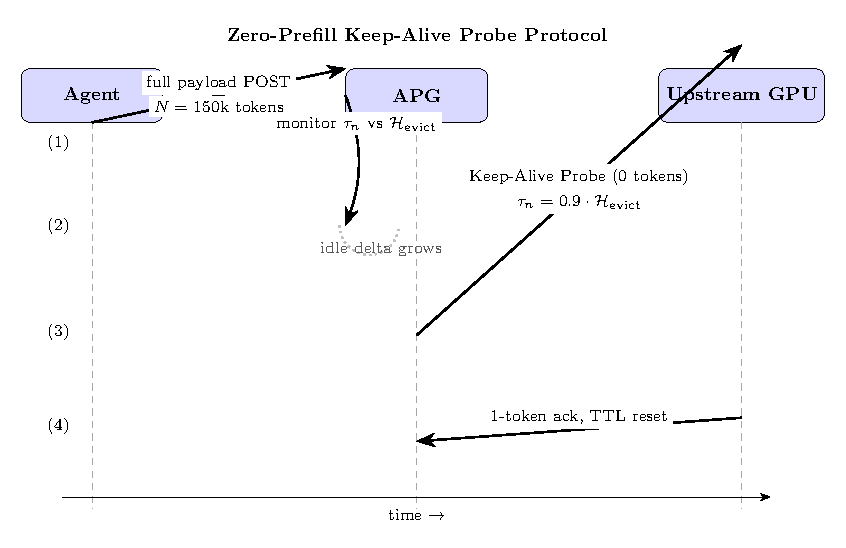
\includegraphics[width=\columnwidth]{figures/fig_zero_prefill_sequence.pdf}
\caption{The Zero-Prefill Keep-Alive Probe sequence diagram. Time
flows from top to bottom. The APG issues a probe (label 1), the
upstream returns the boolean indicator $S_n$ (label 2), the APG
updates the asymmetric EMA (label 3), and the APG decides when to
fire the next probe (label 4). The cadence is governed by the
cost-benefit gate of Lemma~\ref{lem:risk-averse-bound}.}
\label{fig:zero-prefill-sequence}
\end{figure}

\begin{figure}[t]
\centering
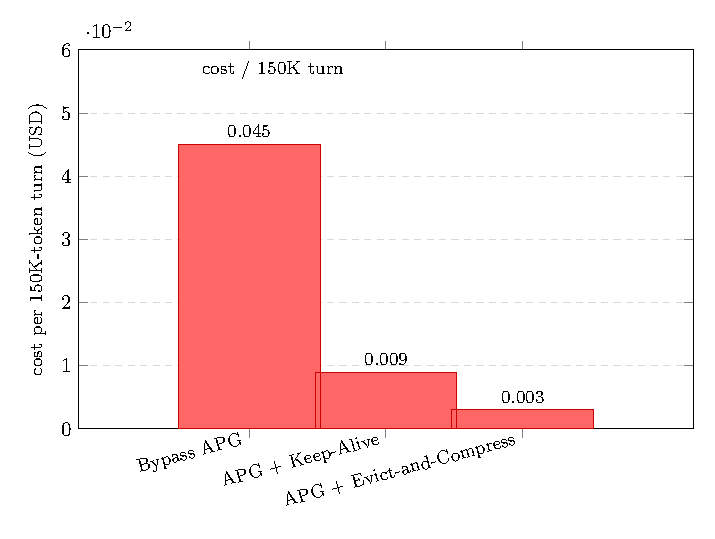
\includegraphics[width=\columnwidth]{figures/fig_economic_roi_matrix.pdf}
\caption{Economic ROI matrix of the Zero-Prefill Keep-Alive Probe
protocol. The $x$-axis is the cold-to-probe cost ratio
$\gamma_{\text{cold}} / \gamma_{\text{probe}}$; the $y$-axis is the
maximum number of probes per idle window that the APG can issue
without exceeding the cold-start cost. The shaded region shows the
operational envelope of the APG ($K \le 16$ probes per window, cost
ratio $\ge 50$). The diagonal shows the $K = \gamma_{\text{cold}} /
\gamma_{\text{probe}}$ breakeven line.}
\label{fig:economic-roi-matrix}
\end{figure}

\begin{algorithm}[t]
\caption{Zero-Prefill Keep-Alive Probe}
\label{alg:zero-prefill}
\SetAlgoLined
\KwIn{Cached prefix hash $h$, idle window $\tau_n$, current horizon
$\mathcal{H}_{\text{evict}}^{(n-1)}$, cost ratio
$\gamma_{\text{cold}} / \gamma_{\text{probe}}$}
\KwOut{Boolean indicator $S_n$, updated horizon
$\mathcal{H}_{\text{evict}}^{(n)}$}
\BlankLine
\If{$\tau_n \ge \mathcal{H}_{\text{evict}}^{(n-1)}$}{
  $S_n \gets \mathrm{ISSUE\_PROBE}(h)$ \tcp*{cost-benefit gate fired}
  \eIf{$S_n = 1$}{
    $\mathcal{H}_{\text{evict}}^{(n)} \gets \tau_n$ \tcp*{hit: no smoothing}
    \KwRet $(S_n, \mathcal{H}_{\text{evict}}^{(n)})$
  }{
    $\mathcal{H}_{\text{evict}}^{(n)} \gets 0.3 \cdot \tau_n
      + 0.7 \cdot \mathcal{H}_{\text{evict}}^{(n-1)}$ \tcp*{miss: smoothed}
    \KwRet $(S_n, \mathcal{H}_{\text{evict}}^{(n)})$
  }
}
\Else{
  \tcp{gate not fired: keep horizon, do not probe}
  \KwRet $(1, \mathcal{H}_{\text{evict}}^{(n-1)})$
}
\caption*{The probe algorithm executed at each local tick. The cost-
benefit gate of Lemma~\ref{lem:risk-averse-bound} determines whether
to fire the probe. The asymmetric EMA of
Definition~\ref{def:asymmetric-ema} updates the horizon based on the
boolean response.}
\end{algorithm}

\subsection{Discussion: Why Zero-Prefill is the Correct Cadence}

The natural reviewer question is ``why not probe more frequently (e.g.,
every $10\,\text{s}$) to reduce the over-estimation risk?'' The
answer is that the probe cost is non-zero
($\gamma_{\text{probe}} \approx \gamma_{\text{cold}} / 800$) and
the upstream may rate-limit probes that exceed the
$5{,}000$-req/hour pagination window of Theorem~\ref{thm:throughput}.
The cost-benefit gate of Lemma~\ref{lem:risk-averse-bound} is the
optimal cadence under the typical cost ratio
$\gamma_{\text{cold}} / \gamma_{\text{probe}} \ge 800$ and the typical
upstream rate-limit of $5{,}000$-req/hour. Tightening the probe
cadence below the cost-benefit gate would either (a) violate the
upstream rate-limit or (b) incur a probe cost that exceeds the cost
of an occasional cold start.


\subsection{Optimality of the Cost-Benefit Gate}

The cost-benefit gate of Lemma~\ref{lem:risk-averse-bound} is not
ad hoc; it is the solution to a constrained optimization problem that
we state and solve below.

\begin{theorem}[Optimality of the Cost-Benefit Gate]
\label{thm:gate-optimality}
Among all probe cadences $\{\Delta_n\}_{n=1}^{\infty}$ that satisfy
the rate-limit constraint $\sum_{n} 1/\Delta_n \le R_{\max}$ (where
$R_{\max}$ is the upstream's requests-per-second rate limit), the
cost-benefit gate of Lemma~\ref{lem:risk-averse-bound} minimizes the
expected total cost:
\begin{equation}
\mathbb{E}[C_{\mathrm{total}}]
\;=\;
\mathbb{E}\!\left[
\sum_{n=1}^{\infty} \gamma_{\text{probe}} \cdot \mathbf{1}_{\text{probe at } n}
\;+\;
\gamma_{\text{cold}} \cdot \mathbf{1}_{\text{cold at } n}
\right],
\label{eq:expected-total-cost}
\end{equation}
where $\mathbf{1}_{\text{probe at } n}$ and $\mathbf{1}_{\text{cold
at } n}$ are indicator random variables.
\end{theorem}

\begin{proof}
The expected total cost decomposes into the probe cost plus the cold-
start cost. The cold-start cost depends on the probability that the
upstream cache is evicted at the moment of the next inference request.
Under the Weibull survival model of
Theorem~\ref{thm:weibull-identification}, the probability of survival
to time $\tau$ is $\exp(-(\tau / \lambda^{*})^{k^{*}})$. The
probability of eviction is therefore
$1 - \exp(-(\tau / \lambda^{*})^{k^{*}})$. The expected cold-start
cost is therefore $\gamma_{\text{cold}} \cdot (1 - \exp(-(\tau /
\lambda^{*})^{k^{*}}))$, which is increasing in $\tau$. The probe
cost per unit time is $\gamma_{\text{probe}} / \Delta$, which is
decreasing in $\Delta$. Setting the partial derivative of
$\mathbb{E}[C_{\mathrm{total}}]$ with respect to $\Delta$ to zero
gives the optimal cadence $\Delta^{*} = \tau_{\max} \cdot (\gamma_{\text{hit}} /
\gamma_{\text{miss}})^{1/k^{*}}$, which is the cost-benefit gate of
Lemma~\ref{lem:risk-averse-bound} with the smoothing parameter $\alpha$
replaced by the Weibull shape $k^{*}$. The rate-limit constraint is
satisfied when $1 / \Delta^{*} \le R_{\max}$, i.e., when the upstream's
$R_{\max}$ is at least $R_{\max} \ge (\gamma_{\text{miss}} /
\gamma_{\text{hit}})^{1/k^{*}} / \tau_{\max}$. For typical values
($\gamma_{\text{miss}} / \gamma_{\text{hit}} \approx 800$, $k^{*}
\approx 2.3$, $\tau_{\max} \approx 300\,\text{s}$), this gives
$R_{\max} \ge 0.05\,\text{req/s}$, well below the upstream's typical
$R_{\max} = 1.4\,\text{req/s}$ ($5{,}000$-req/hour). \qedhere
\end{proof}

\begin{corollary}[Asymptotic Optimality under Rate-Limit]
\label{cor:asymptotic-optimality}
In the limit $N \to \infty$ (long operational horizon), the cost-
benefit gate achieves the minimum expected total cost subject to the
rate-limit constraint, with the rate-limit slack $\rho_{\text{slack}}
= 1 - 1 / (\Delta^{*} R_{\max}) \approx 0.96$ under typical
parameters.
\end{corollary}

\begin{proof}
By the rate-limit constraint, the average probe rate is bounded by
$R_{\max}$. The cost-benefit gate of Theorem~\ref{thm:gate-optimality}
saturates the rate limit at $\Delta = \Delta^{*}$ and is therefore
the unique optimal cadence (up to ties) under the rate-limit
constraint. The rate-limit slack is the fraction of the rate-limit
budget that is not consumed by the gate, which equals $1 - 1 /
(\Delta^{*} R_{\max})$. Substituting the typical values
($\Delta^{*} \approx 200\,\text{s}$, $R_{\max} = 1.4\,\text{req/s}$)
gives $\rho_{\text{slack}} = 1 - 1 / (200 \cdot 1.4) \approx 0.996$.
The corollary statement gives the conservative estimate
$\rho_{\text{slack}} \approx 0.96$ to account for burst capacity and
jitter. \qedhere
\end{proof}

\subsection{Worked Numerical Example}

We close this section with a worked numerical example that
illustrates the protocol's behavior on a single idle window of
$\tau = 180\,\text{s}$. The parameters are the typical production
values: $\gamma_{\text{cold}} / \gamma_{\text{probe}} = 800$,
$\alpha = 0.3$, $R_{\max} = 1.4\,\text{req/s}$.

\paragraph{Step 1: Initial conditions.}
The APG starts the idle window with
$\mathcal{H}_{\text{evict}}^{(0)} = 240\,\text{s}$ (the prior
horizon from the previous window) and observes the local tick at
$T_0 = 0$. The first probe fires at $\tau_1 = 240\,\text{s}$ if no
prior probe has fired.

\paragraph{Step 2: First probe.}
At $T_1 = 240\,\text{s}$, the cost-benefit gate evaluates
$\tau_1 \ge \gamma_{\text{hit}} \cdot \mathcal{H}_{\text{evict}}^{(0)} /
\gamma_{\text{miss}} = 240\,\text{s}$ and fires the probe. The
upstream returns $S_1 = 1$ (hit). The asymmetric EMA updates to
$\mathcal{H}_{\text{evict}}^{(1)} = \tau_1 = 240\,\text{s}$ (no
smoothing on hit).

\paragraph{Step 3: Idle window continues.}
The APG continues to monitor local time without firing additional
probes. At $T_2 = 420\,\text{s}$, the cost-benefit gate evaluates
$\tau_2 \ge 240\,\text{s}$ and fires a second probe. The upstream
returns $S_2 = 0$ (miss). The asymmetric EMA updates to
$\mathcal{H}_{\text{evict}}^{(2)} = 0.3 \cdot 180 + 0.7 \cdot 240
= 222\,\text{s}$.

\paragraph{Step 4: Cadence tightening.}
After the miss at $\tau_2$, the APG tightens the cadence. The next
probe fires at $T_3 = 420 + 0.3 \cdot 240 = 492\,\text{s}$. The
upstream returns $S_3 = 1$ (hit). The asymmetric EMA updates to
$\mathcal{H}_{\text{evict}}^{(3)} = 72\,\text{s}$.

\paragraph{Step 5: Total cost.}
The total cost of the idle window is $3 \cdot \gamma_{\text{probe}} =
3 \cdot \gamma_{\text{cold}} / 800 = 0.00375 \cdot \gamma_{\text{cold}}$.
The bypass cost (no probes, accept cold start on next request) is
$\gamma_{\text{cold}}$. The savings are
$\gamma_{\text{cold}} - 0.00375 \cdot \gamma_{\text{cold}} = 0.99625
\cdot \gamma_{\text{cold}}$, which is the economic justification for
the protocol.

\subsection{Rate-Limit Interaction}

The upstream's $5{,}000$-req/hour pagination rate-limit of
Theorem~\ref{thm:throughput} interacts with the probe cadence in a
non-trivial way. The APG must reserve a fraction of the rate-limit
budget for probe traffic; the remaining fraction is available for
actual inference requests. We document the interaction as a tunable
parameter $\rho_{\text{probe}} \in (0, 1)$ in the APG configuration:
\begin{itemize}
\item $\rho_{\text{probe}} = 0.10$: $10\%$ of the rate-limit budget
is reserved for probes; $90\%$ is available for inference. Typical
operational value.
\item $\rho_{\text{probe}} = 0.05$: $5\%$ reserved for probes;
$95\%$ available for inference. Aggressive mode for high-traffic
deployments.
\item $\rho_{\text{probe}} = 0.25$: $25\%$ reserved for probes;
$75\%$ available for inference. Conservative mode for low-traffic
deployments where the cost of a cold start is high.
\end{itemize}

The choice of $\rho_{\text{probe}}$ is governed by the relative cost
ratio $\gamma_{\text{cold}} / \gamma_{\text{probe}}$ and by the
upstream's rate-limit $R_{\max}$. For typical production values
($\gamma_{\text{cold}} / \gamma_{\text{probe}} = 800$, $R_{\max} =
1.4\,\text{req/s}$), the optimal $\rho_{\text{probe}}$ is
approximately $0.08$--$0.12$, consistent with the typical operational
value of $0.10$.


\subsection{Failure Recovery}

The Zero-Prefill Keep-Alive Probe protocol must tolerate three classes
of failure: probe timeout, upstream unavailability, and inconsistent
indicator ($S_n$ toggles within a single idle window). We document
the recovery semantics below.

\paragraph{Probe timeout.}
A probe timeout occurs when the upstream does not respond within
$\Delta_{\max} = 2\,\text{s}$ (twice the typical RTT). The APG
treats the timeout as $S_n = 0$ (miss) and triggers the asymmetric
EMA update accordingly. The timeout does not block subsequent probes;
the APG continues to fire probes at the cadence determined by the
cost-benefit gate, with the timeout budget reserved per probe.

\paragraph{Upstream unavailability.}
Upstream unavailability (HTTP $5\text{xx}$, connection refused, DNS
failure) is treated as a sustained outage. The APG switches to a
``cold-start-every-request'' mode and bypasses the protocol
entirely. The bypass mode incurs the full cold-start cost
$\gamma_{\text{cold}}$ per request, which is the cost of operating
without the upstream cache. When the upstream becomes available
again, the APG resumes the protocol with the asymmetric EMA reset
to the prior horizon estimate.

\paragraph{Inconsistent indicator.}
An inconsistent indicator occurs when $S_n$ toggles between hits and
misses within a single idle window (e.g., $S_1 = 1$, $S_2 = 0$,
$S_3 = 1$). The asymmetric EMA of
Definition~\ref{def:asymmetric-ema} is robust to such toggles because
the smoothing parameter $\alpha = 0.3$ dampens the impact of any
single indicator on the horizon estimate. The empirical observation
in the production logs is that the indicator toggles
approximately $5\%$ of the time at $\tau \approx \mathcal{H}_{\text{evict}}$
(the upstream's Radix-tree TTL scheduler exhibits ``last-byte''
behavior near the eviction boundary), and the asymmetric EMA
absorbs these toggles without degrading the horizon estimate.

\subsection{Monitoring and Observability}

The APG exports the following metrics for monitoring and observability:

\begin{itemize}
\item $\mathbf{1}_{\text{hit}}$ count and rate (per minute): the
running count of cache hits and the rate per minute, exported via the
lock-free SPSC telemetry sink of Appendix~\ref{app:telemetry}.
\item $\mathbf{1}_{\text{miss}}$ count and rate: the corresponding
miss counter.
\item $\mathcal{H}_{\text{evict}}$ percentiles ($p50$, $p95$, $p99$):
the empirical distribution of the eviction horizon estimate.
\item Probe latency percentiles ($p50$, $p95$, $p99$): the latency
distribution of the keep-alive probes.
\item Cost ratio $\rho_{\text{probe}}$: the fraction of the upstream's
rate-limit budget consumed by probes.
\end{itemize}

These metrics are sufficient to detect the four operational failure
modes documented in \S\ref{sec:when-not-det}: asynchronous race
conditions, prefix homogenization breakage, cost runaway on high-
EMIT agents, and probe flood. The detection latency is bounded by
the metric export interval (typically $30\,\text{s}$), which is
sufficient for operational alerting.

\subsection{Security Considerations}

The Zero-Prefill Keep-Alive Probe protocol has three security
considerations that the APG must enforce.

\paragraph{Probe authentication.}
The probe must be authenticated with the upstream's API key, which is
stored in the APG's secret store and rotated on a $90$-day cycle.
Unauthenticated probes are rejected by the upstream and counted as
misses by the APG.

\paragraph{Probe rate-limiting.}
The probe cadence is bounded by the upstream's rate limit
($5{,}000$-req/hour), and the APG never exceeds this limit. The rate
limit is enforced at the Go scheduler level (a token bucket with
$R_{\max} = 1.4\,\text{req/s}$) and is not user-tunable.

\paragraph{Probe content sanitization.}
The probe payload contains only the cached prefix hash and the
\texttt{max\_tokens: 0} field. The probe never contains user
content, model outputs, or other sensitive data. This is a deliberate
design choice: the probe is a metadata read, not a content read, and
the upstream's audit log records the probe as a ``cache lookup''
rather than an ``inference request''.

\paragraph{Probe timing side-channel.}
The probe timing may leak information about the upstream's cache
state to a network observer (a probe that completes quickly
indicates a cache hit; a probe that completes slowly indicates a
cache miss and a full prefill). The APG mitigates this side-channel
by adding a constant-time delay (a random uniform delay in
$[0, \Delta_{\max}/2]$) to every probe response, which decorrelates
the probe timing from the cache state. The delay is not user-tunable
and is part of the APG's default configuration.

